% Fig A — federation architecture (paper.md, §Executable contract surface).
% TikZ standalone (tikz + standalone only).
% Regenerate the committed PDF: make figures-architecture

\documentclass[border=6pt]{standalone}
\usepackage{tikz}
\usetikzlibrary{positioning, arrows.meta, calc}

\begin{document}
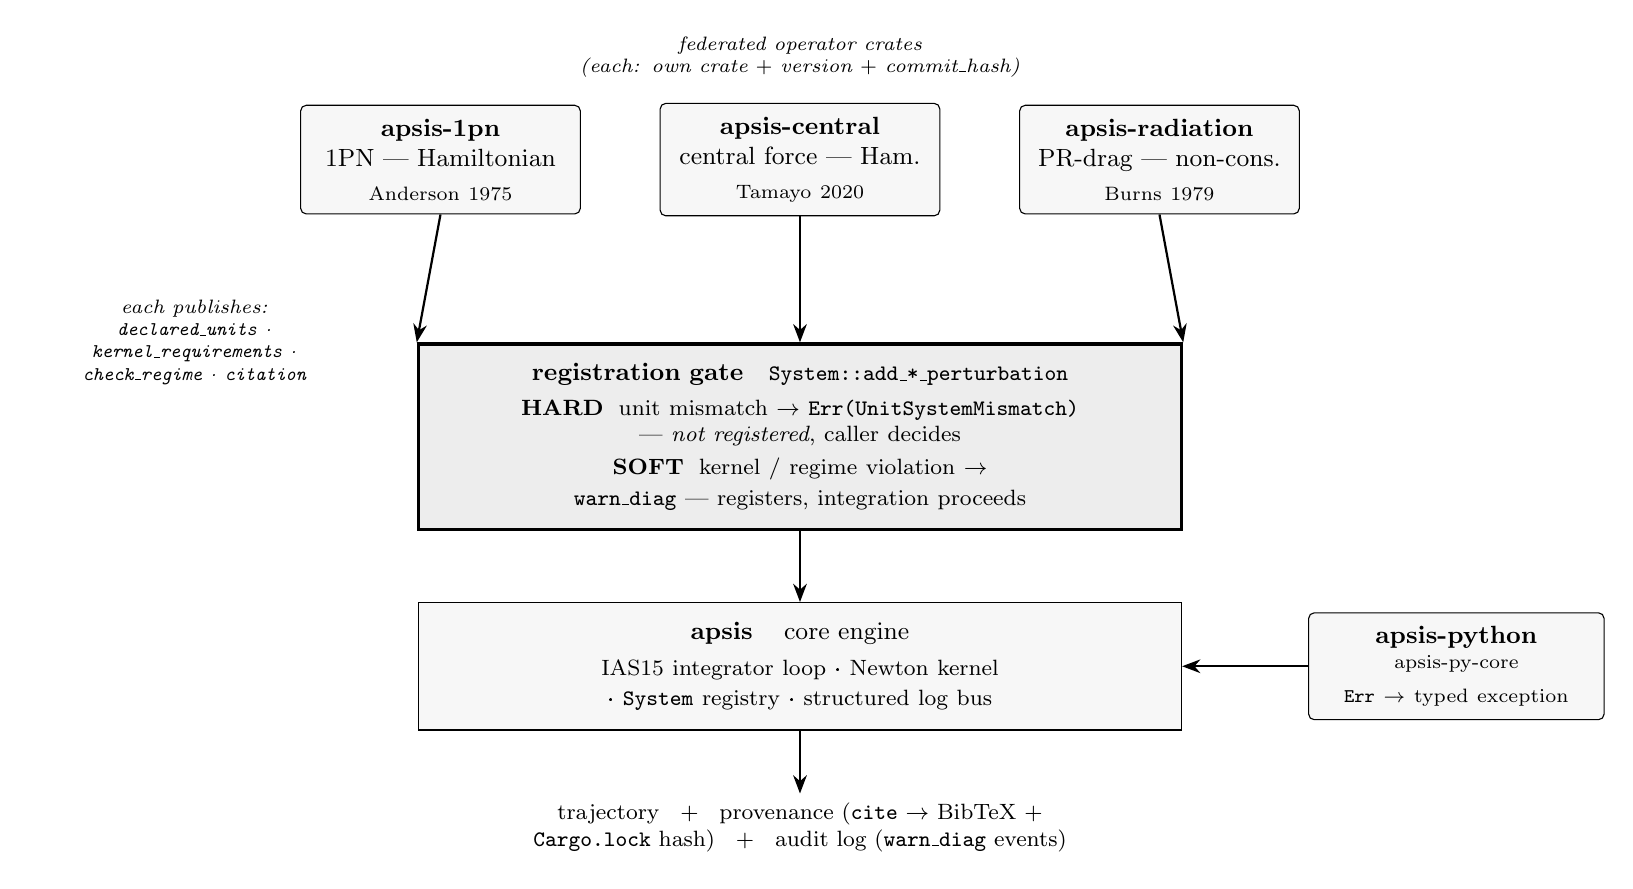
\begin{tikzpicture}[
    font=\small,
    >=Stealth,
    crate/.style={draw, rounded corners=2pt, align=center, fill=black!3,
                  inner sep=5pt, minimum height=13mm, text width=32mm},
    gate/.style={draw, very thick, align=center, fill=black!7,
                 inner sep=7pt, text width=92mm},
    core/.style={draw, align=center, fill=black!3, inner sep=7pt, text width=92mm},
    io/.style={align=center, text width=105mm, font=\footnotesize},
    note/.style={align=center, font=\scriptsize\itshape, text width=86mm},
    arr/.style={->, thick},
]

% ── federated operator crates (top row) ──────────────────────────────────────
\node[crate] (pn) {\textbf{apsis-1pn}\\1PN — Hamiltonian\\[1pt]\scriptsize Anderson 1975};
\node[crate, right=10mm of pn] (cf)
    {\textbf{apsis-central}\\central force — Ham.\\[1pt]\scriptsize Tamayo 2020};
\node[crate, right=10mm of cf] (rad)
    {\textbf{apsis-radiation}\\PR-drag — non-cons.\\[1pt]\scriptsize Burns 1979};

\node[note, above=2mm of cf] (crates-label)
    {federated operator crates\\(each: own crate $+$ version $+$ commit\_hash)};

% ── registration gate (focal point) ─────────────────────────────────────────
\node[gate, below=16mm of cf] (gate)
    {\textbf{registration gate}\quad\texttt{\footnotesize System::add\_*\_perturbation}\\[3pt]
     \footnotesize \textbf{HARD}\; unit mismatch $\to$ \texttt{Err(UnitSystemMismatch)} —
     \emph{not registered}, caller decides\\[1pt]
     \footnotesize \textbf{SOFT}\; kernel / regime violation $\to$ \texttt{warn\_diag} —
     registers, integration proceeds};

% ── publishes annotation (clear to the left of the gate's top-left corner) ───
\node[note, text width=40mm, anchor=east] (pub) at ([xshift=-7mm]gate.north west)
    {each publishes:\\ \texttt{declared\_units} · \texttt{kernel\_requirements} ·
     \texttt{check\_regime} · \texttt{citation}};

% ── core engine ──────────────────────────────────────────────────────────────
\node[core, below=9mm of gate] (core)
    {\textbf{apsis} \;\; core engine\\[2pt]
     \footnotesize IAS15 integrator loop · \mbox{Newton kernel} · \texttt{System} registry ·
     \mbox{structured log bus}};

% ── outputs ──────────────────────────────────────────────────────────────────
\node[io, below=8mm of core] (out)
    {trajectory \;\;$+$\;\; provenance (\texttt{cite} $\to$ BibTeX $+$ \texttt{Cargo.lock} hash)
     \;\;$+$\;\; audit log (\texttt{warn\_diag} events)};

% ── Python binding (consumer surface, to the side) ───────────────────────────
\node[crate, text width=34mm, right=16mm of core] (py)
    {\textbf{apsis-python}\\[1pt]\scriptsize apsis-py-core\\[1pt]
     \scriptsize \texttt{Err} $\to$ typed exception};

% ── edges ────────────────────────────────────────────────────────────────────
\draw[arr] (pn.south)  -- (gate.north west);
\draw[arr] (cf.south)  -- (gate.north);
\draw[arr] (rad.south) -- (gate.north east);
\draw[arr] (gate) -- (core);
\draw[arr] (core) -- (out);
\draw[arr] (py.west) -- (core.east);

\end{tikzpicture}
\end{document}
